\newcommand{\flexible}{\em{Flexible}}

\newcommand{\pos}{\vect{x}}
\newcommand{\dx}{\vect{\Delta x}}
\newcommand{\xcur}{\vect{x}_{n}}
\newcommand{\xnext}{\vect{x}_{n+1}}
\newcommand{\vel}{\vect{v}}
\newcommand{\dv}{\vect{\Delta v}}
\newcommand{\vcur}{\vect{v}_{n}}
\newcommand{\vnext}{\vect v_{n+1}}
\newcommand{\acc}{\vect{a}}
\newcommand{\force}{\vect{f}}
\newcommand{\forcext}{\vect{f}_{ext}}
\newcommand{\lam}{\vect{\lambda}}
\newcommand{\lcur}{\lam_{n}}
\newcommand{\lnext}{\lam_{n+1}}
\newcommand{\avlam}{\bar{\lam}}
\newcommand{\fcur}{\vect{f}_{n}}
\newcommand{\fnext}{\vect f_{n+1}}
\newcommand{\Minv}{\mat M^{-1}}
\renewcommand{\P}{\mat P}
\newcommand{\cmp}{c}
\newcommand{\dampingratio}{d}

\newcommand{\p}{\vect{p}}  % moving point
\newcommand{\polynomial}[2]{{#1}^{#2}}  % polynomial coordinates of a point
\newcommand{\pp}{\polynomial{\p}{*}}  % polynomial coordinates of point p
\newcommand{\ppinit}{\polynomial{\pinit}{*}}  % polynomial coordinates of point \bar p
\newcommand{\initial}[1]{\bar{#1}}  % initial coordinates of a point
\newcommand{\pinit}{\initial{\p}}  % initial coordinates of a point
\newcommand{\pref}{\initial{\p}}  % reference (undeformed) point
\newcommand{\disp}{\vect{u}}  % displacement
\newcommand{\f}{\vect{f}}    % forces

\newcommand{\dof}{q}           % independent DOF
\newcommand{\dofinit}{\initial\dof}           % independent DOF
\newcommand{\dofpos}{\ensuremath{\vect{x}} }           % posititon in 3d of an independent DOF
\newcommand{\dofposinit}{\initial\dofpos }           % posititon in 3d of an independent DOF
\newcommand{\pdofposinit}{\polynomial{\dofposinit}{*}}
\newcommand{\pdofposinitcov}[1]{\polynomial{\dofposinit_#1}{*}\polynomial{\dofposinit_#1}{*T}}
\newcommand{\vdof}{\vect{\dof}}           % vector of independent DOF
\newcommand{\vdofinit}{\vect{\dofinit}}          % independent DOF
\newcommand{\fdof}{\f}           % force on independent DOF
\newcommand{\vfdof}{\vect{\fdof}}           % vector of independent DOF force
\newcommand{\dofm}{\mat{A}}         % DOF matrix
\newcommand{\dofmrel}{\mat{A^r}}         % DOF matrix
\newcommand{\mparam}{\theta}           % material parameter
\newcommand{\vmparam}{\vect{\mparam}}           % material points
\newcommand{\defograd}{F}           % deformation gradient
\newcommand{\strain}{\epsilon}           % strain
\newcommand{\stress}{\sigma}           % stress
\newcommand{\W}{\mathcal{W}}           % elastic energy
\newcommand{\C}{\mat{C}}           % damping matrix

\newcommand{\volume}{\ensuremath{\mathcal{V}}} 
\newcommand{\sample}{\ensuremath{{\mathcal{V}e}}} 
\newcommand{\vol}{\ensuremath{\Delta v}}
\newcommand{\volmass}{\ensuremath{\rho}}
\newcommand{\mass}{\mat{M}}

\newcommand{\ddof}{\ensuremath{\dot{\dof}}}
\newcommand{\dddof}{\ensuremath{\ddot{\dof}}}
\newcommand{\diff}{\ensuremath{\boldsymbol{\nabla}_i}}

\newcommand{\Jt}{\J^T}

\newcommand{\mCoord}{\vect{\Theta}}
\newcommand{\shapef}{w}

\newcommand{\MappingArrows}{\ensuremath{\left. \begin{array}{c} \stackrel{\JNL}{\longrightarrow} \\ \stackrel{\J}{\longrightarrow} \\ \stackrel{\Jt}{\longleftarrow} \end{array}\right.} }

\begin{abstract}
This plugin provides a unified approach to the simulation of deformable solids using mass-spring, FEM and mesh-less models.
New mappings are introduced to compute material deformations based on node positions, and strain from deformations.
FEM and mesh-less models use different position-deformation mappings. The remaining components (strain measures, constitutive laws) are common to the two approaches.
\end{abstract}

\section{Overview}

In this plugin, our goal is to separate each stage of the simulation into individual components to improve the modularity of the simulator.
Figure~\ref{fig modularity mass-spring} shows an example of the increased modularity.
In \sofa{}, mass-spring systems are traditionally modeled using three components for  state, mass and penalty force. 
The force component $F_s$ in fig.\ref{fig mass-spring-traditional} is in charge of computing the distance and its gradient between the two particles, as well as to apply a constitutive law (typically linear viscoelastic).
In this plugin, we provide new components to split these computations and make the framework more modular.
In the example shown in fig.\ref{fig mass-spring-flexible}, a mapping is used to compute spring extensions $X_e$ based on particle positions $X_p$. 
A constitutive law $F_e$ is applied to the extensions, and the corresponding force is mapped upward to the particles through the mapping.
This is more modular since the linear viscoelastic constitutive law can be replaced with a different one, while re-using the same mapping from positions to extensions. In the traditional approach, extension computation would have to be re-implemented in the new force field.
Moreover, in the new approach, the penalty force can also be replaced with a hard constraint, while re-using the same mapping (see also the Compliant plugin about soft and hard constraints).
More generally, complex components cam be decomposed in simple (and re-usable) components using  mappings.
In Flexible, we have leveraged this property to propose a unified approach to the simulation of deformable solids using mass-spring, FEM and mesh-less models.
\begin{figure}
 \centering
 \begin{subfigure}[t]{0.36\linewidth} \centering
   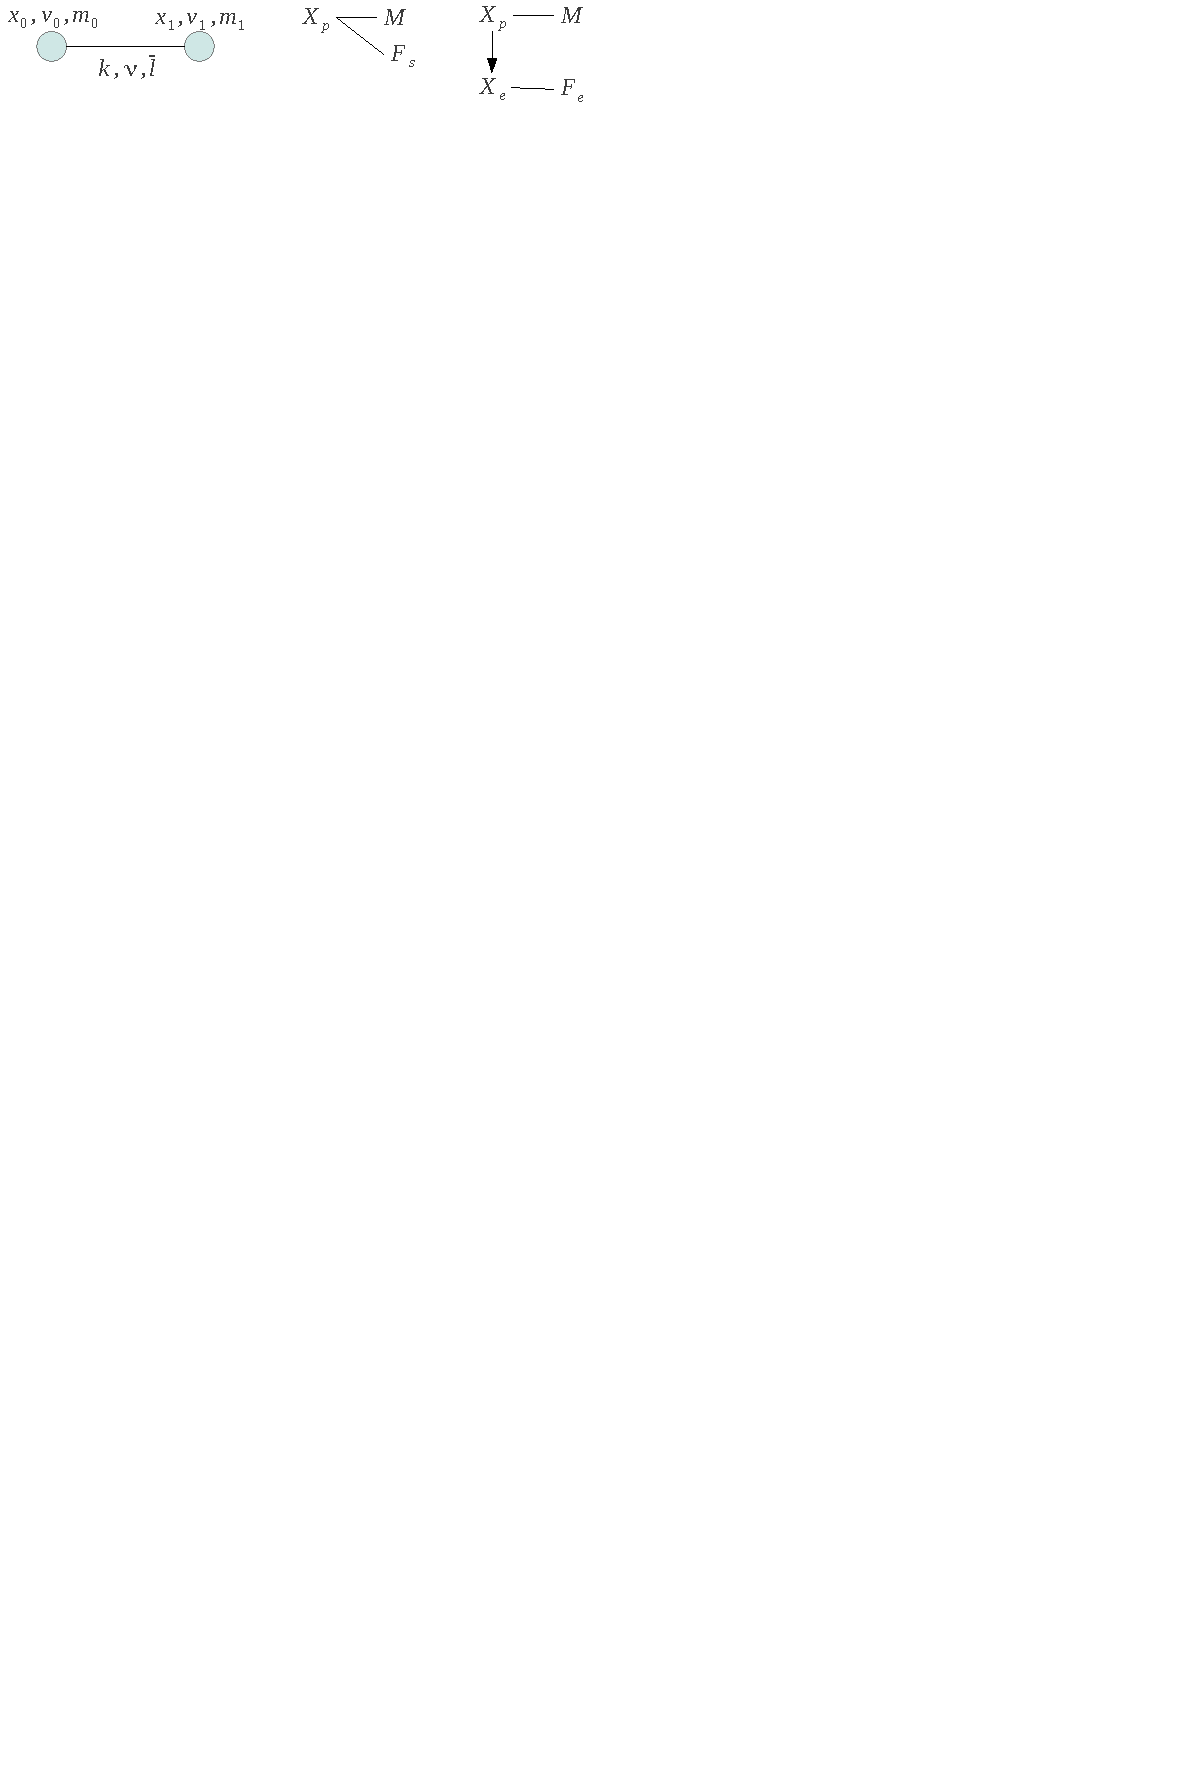
\includegraphics[clip,trim=0mm 285mm 155mm 0mm]{mass-spring.pdf}
   \caption{Two masses and a spring.} \label{fig mass-spring}
 \end{subfigure}
 \begin{subfigure}[t]{0.3\linewidth} \centering
   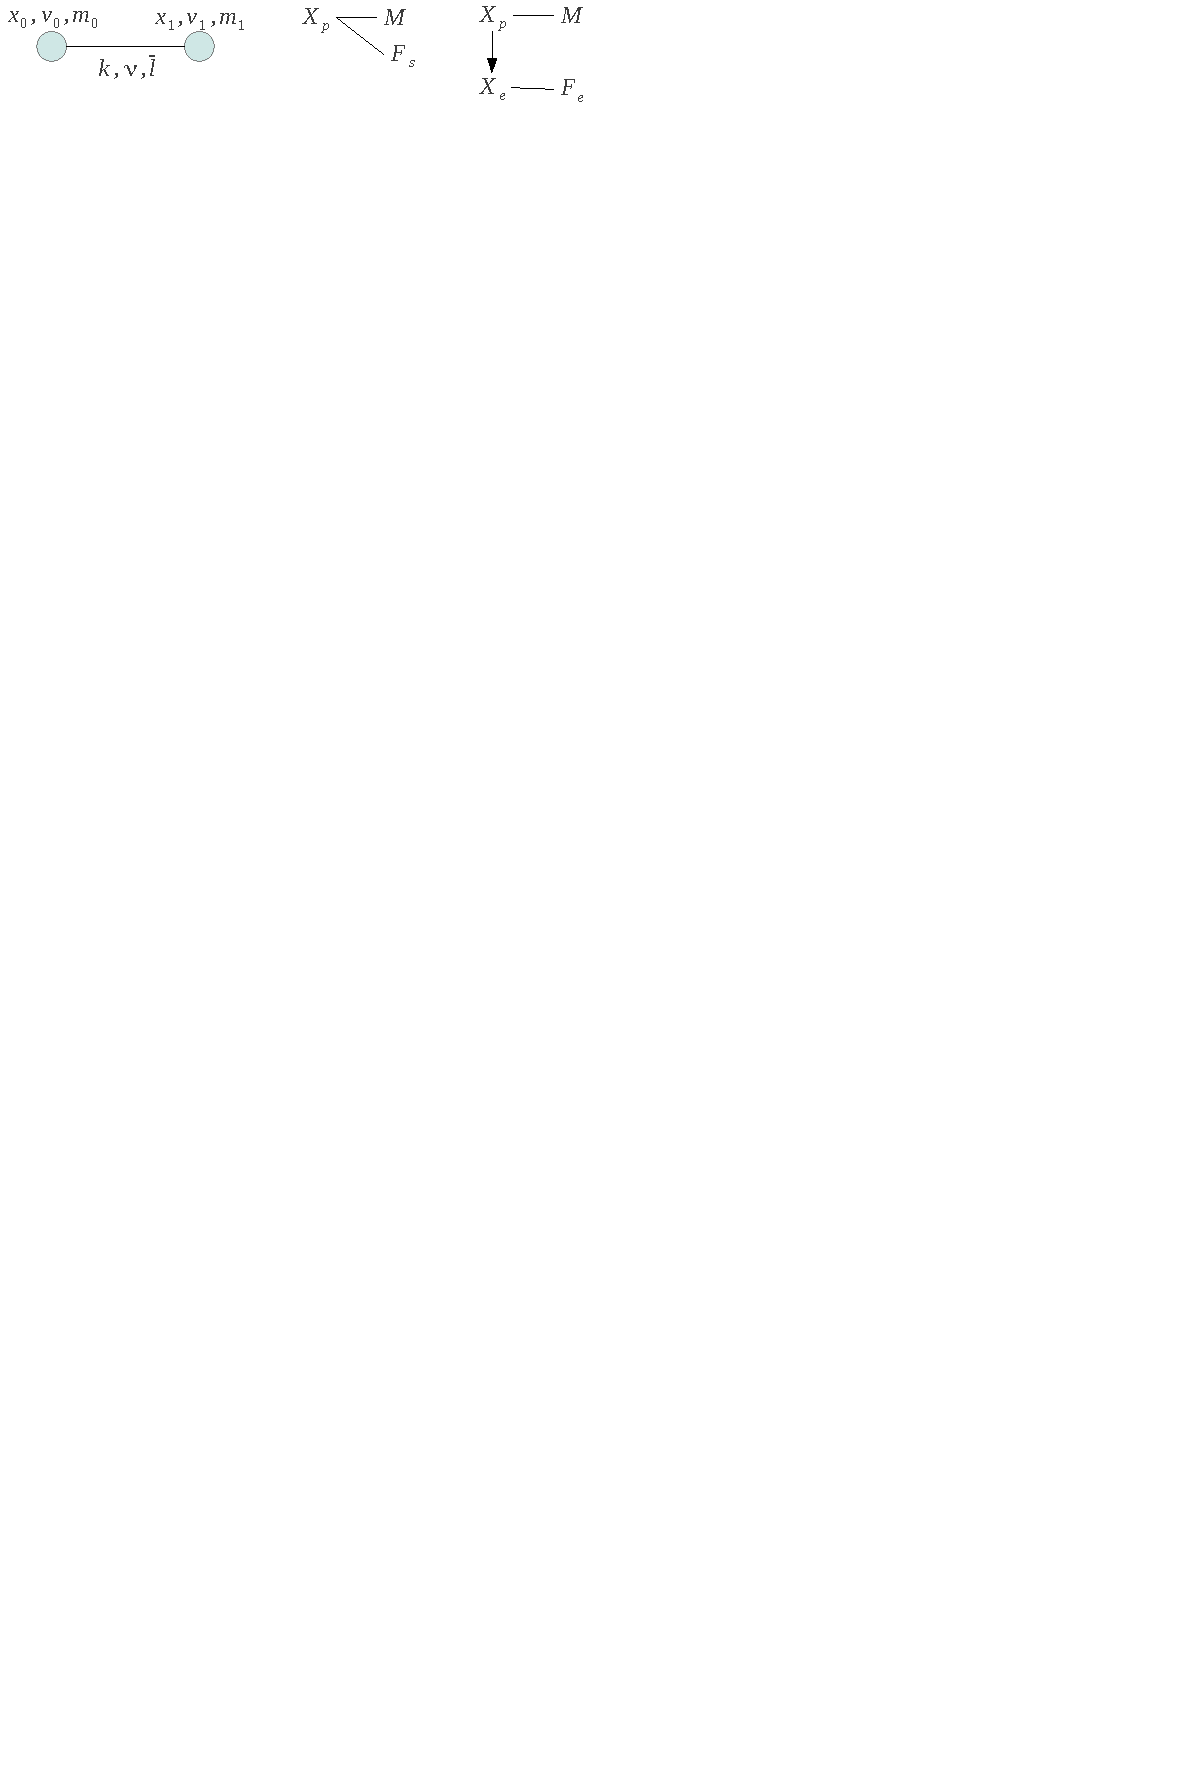
\includegraphics[clip,trim=50mm 285mm 130mm 0mm]{mass-spring.pdf}
   \caption{Traditional \sofa{} scene graph.} \label{fig mass-spring-traditional}
 \end{subfigure}
 \begin{subfigure}[t]{0.3\linewidth} \centering
   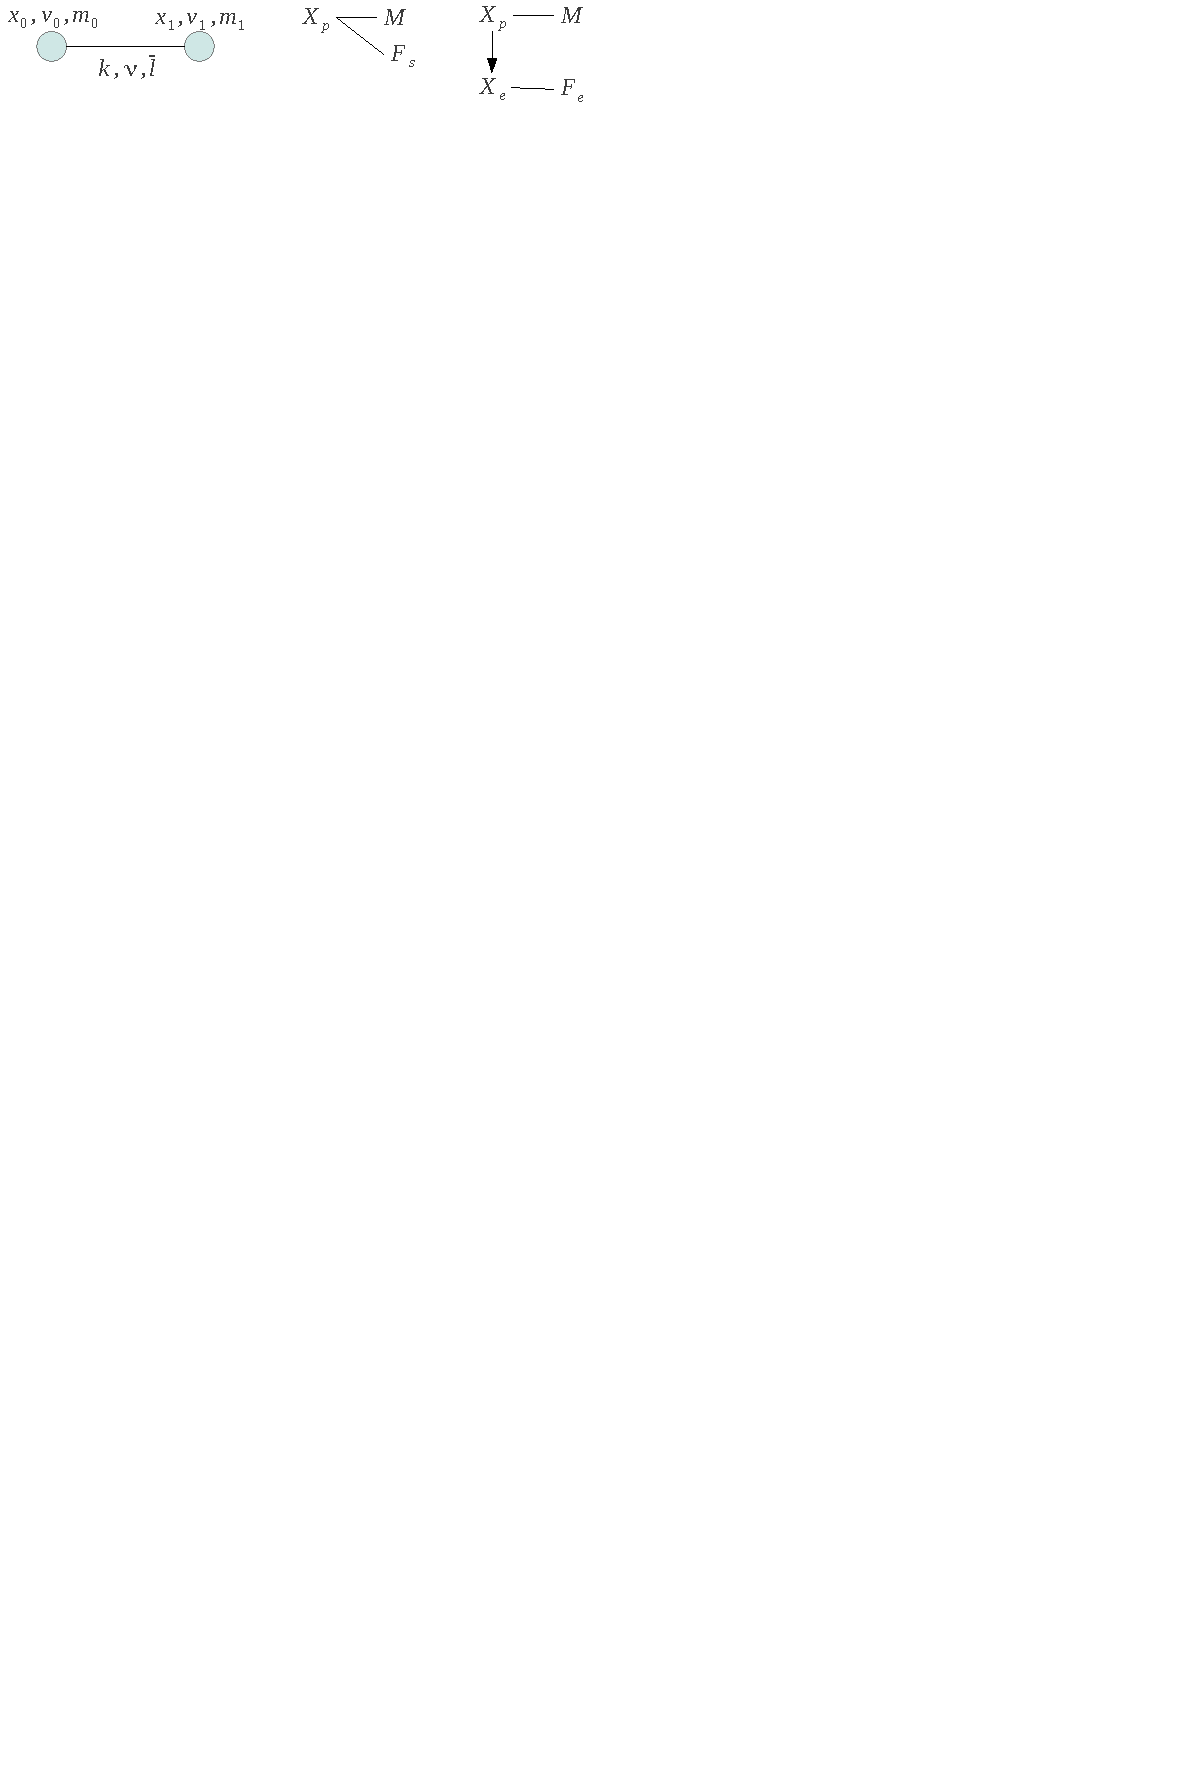
\includegraphics[clip,trim=80mm 280mm 100mm 0mm]{mass-spring.pdf}
   \caption{A more modular data structure.} \label{fig mass-spring-flexible}
 \end{subfigure}
 \caption{Improved modularity. $X$ denotes a state component, $M$ is mass, and $F$ a force field, while arrows represent mappings. $X_p$ represents particle positions while $X_e$ represents spring extensions, and $F_s$ represents spring forces while $F_e$ represent extension forces.}
 \label{fig modularity mass-spring}
\end{figure}


The numerical simulation of continuous deformable objects is based on a discrete number of independent degrees of freedom (DOFs) which we will call the nodes. They are kinematic primitives (can be points, frames, etc.).

Nodes are associated with shape functions which are combined to produce the displacement function of material points in the solid.

We introduce the following notations:
\begin{itemize}
 \item $\vdofinit$, $\vdof$ and $\fdof$ : the initial positions, current positions, and forces of the nodes.
 \item $\mCoord$ : the material coordinates of a point according the chosen parameterization of the solid.
 \item $\pinit(\mCoord)$, $\p (\mCoord)$ : the initial and current position of a point in space
 \item $\disp (\mCoord) =\p-\pinit$ : the displacement of a point
 \item $\shapef_i(\mCoord)$ : the shape function associated with node $i$
\end{itemize}

The local deformation is computed by differentiation with respect to material coordinates. The deformation gradient is: $\defograd = \partial \p / \partial \mCoord$.

The elastic deformation is described using a strain measure based on the deformation gradient. 

These three stages can be modeled using \sofa{} mappings:

\begin{equation}
\left. \begin{array}{ccccc}
\mbox{Nodes}  & \MappingArrows &   \mbox{Deformation gradients} & \MappingArrows &  \mbox{Strains}
\end{array}\right. 
\end{equation}

The elastic potential energy is computed from the strain. 

After spatial integration (quadrature), we obtain associated forces (total stress), that can be back propagated to the nodes using transposed jacobians.

\begin{equation}\label{eq:f}
 \vfdof = - \frac{\partial \W}{\partial \vdof}^T =  - \Jt_0\Jt_1 \int_{\volume} \stress
\end{equation}

Force variations are updated at each mapping by combining material and geometric stiffnesses. For a mapping from $p$ to $c$, we have:

\begin{equation}
 \delta(\vfdof_p) = ( \Jt \K_c \J + \frac{\partial \Jt}{\partial \vdof_p} \vfdof_c ) \delta(\vdof_p) 
\end{equation}

\newpage
%--------------------------------------------------------------------------------------------
\section{Scene graph}

\begin{itemize}
 \item \textbf{State =} nodes
 \item Shape function

 \item \textbf{ELASTICITY:}
  \begin{itemize}
  \item Gauss point sampler
  \item \textbf{State =} deformation gradients
  \item \textbf{Mapping =} deformation mapping

  \item \textbf{MATERIAL:}
    \begin{itemize}
    \item \textbf{State =} strains
    \item \textbf{Force field}
    \item \textbf{Mapping =} strain mapping
    \end{itemize}
  \end{itemize}

 \item \textbf{MASS:}
    \begin{itemize}
    \item \textbf{State =} points 
    \item Mass
    \item \textbf{Mapping =} deformation mapping
    \end{itemize}
 \item \textbf{COLLISION:}
    \begin{itemize}
    \item \textbf{State =} points 
    \item \textbf{Mapping =} deformation mapping
    \end{itemize}
 \item \textbf{VISU:}
    \begin{itemize}
    \item \textbf{State =} points 
    \item \textbf{Mapping =} deformation mapping
    \end{itemize}

\end{itemize}

\newpage
%--------------------------------------------------------------------------------------------
\section{Shape functions}

\subsection{Shepard}

Shepard shape functions correspond to inverse distance weights (\url{http://en.wikipedia.org/wiki/Inverse_distance_weighting}).

They are defined as $\shapef_i(\mCoord)=1/|| \mCoord-\mCoord_i ||^p$ followed by normalization.

\subsection{Barycentric}

Barycentric shape functions are the barycentric coordinates of points inside cells (can be edges, triangles, quads, tetrahedra, hexahedra).
They achieve first order consistency: $\mCoord= \sum \shapef_i \mCoord_i$
 
\subsection{Natural Neighbors}

Natural neighbor interpolants are based on Voronoi diagrams.
Currently, Voronoi diagrams are computed from an image (a rasterized object).

\subsection{to do}

\begin{itemize}
 \item higher order FEM
 \item clarify material vs. spatial coordinates
 \item 
\end{itemize}

\newpage
%--------------------------------------------------------------------------------------------
\section{Deformation mapping}

\subsection{linear mapping}

Child positions are computed as a linear combination of parent node dofs.
For instance, the mapping from points to points is : $\p = \sum_i w_i (\vdof - \vdofinit)$.
The mapping from affine frames to points in homogeneous coordinates is : $\p = \sum_i w_i \vdof \vdofinit^{-1} \pinit$.

\subsection{Extension mapping}

\subsection{Distance mapping}

\subsection{Log rigid mapping}

\subsection{Relative rigid mapping}

\subsection{Triangle deformation mapping}

\subsection{to do}

\begin{itemize}
 \item Moving Least squares
 \item non-linear skinning
 \item clarify material vs. spatial coordinates
 \item model plasticity/control using relative mappings
 \item 
\end{itemize}

\newpage
%--------------------------------------------------------------------------------------------
\section{Strain mapping}

\subsection{Green-Lagrangian strain}

The strain is mapped from the deformation gradient as : $\mat{E} = (\defograd^T\defograd - \mat{I} )/2$.
Here the strain is stored into vectors using Voigt notation. In 3d, we have: $\strain = [\strain_{xx} , \strain_{yy} , \strain_{zz} , 2\strain_{xy} , 2\strain_{yx} , 2\strain_{xz} ] $
The energy conjugate SPK stress vector is $\stress = [\stress_{xx} , \stress_{yy} , \stress_{zz} , \stress_{xy} , \stress_{yx} , \stress_{xz} ] $

\subsection{Corotational strain}

The rigid displacement $\mat{R}$ is first extracted from the deformation gradient using, for instance, SVD, polar or QR decomposition.
Then, supposing that the non-rigid deformation $\mat{R}^T \defograd$ is small enough, we can apply the Cauchy strain formulation:  $\mat{E} = [\mat{R}^T \defograd + \defograd^T \mat{R} ) /2 - \mat{I} $.


The geometric stiffness contribution does not seem necessary because it does not visually change the behaviour but can compromise the stability.
\begin{itemize}
\item analytical QR decomposition jacobians given in "Finite Random Matrix Theory, Jacobians of Matrix Transforms (without wedge products)", Alan Edelman, 2005, http://web.mit.edu/18.325/www/handouts/handout2.pdf (UNSTABLE)
\item Polar decomposition gradients inspired by Jernej Barbic, Yili Zhao, "Real-time Large-deformation Substructuring" SIGGRAPH 2011 (UNSTABLE)
\item SVD gradients given in Christopher Twigg, Zoran Kacic-Alesic, "Point Cloud Glue: Constraining simulations using the Procrustes transform", SCA'10 (QUITE STABLE)
\end{itemize}

\subsection{Principal stretches}

The principles streches $\mat{U}$ are directly extracted from the deformation gradient using a SVD, where the principal streches can be deduce from the eigen-values.
Note that the corresponding stress is also represented by 3 values, so isotropic materials are not applicable.

The geometric stiffness contribution is important.
\begin{itemize}
\item SVD gradients given in T. Papadopoulo, M.I.A. Lourakis, "Estimating the Jacobian of the Singular Value Decomposition: Theory and Applications", European Conference on Computer Vision, 2000 (STABLE)
\end{itemize}

\subsection{Diagonal strain}

The diagonal strain $\mat{D}$ is the principles streches + additional terms to allow anisotropic materials. 


\subsection{Invariants of deformation tensor}

The elastic energy of some materials are expressed using the three invariants of the right Cauchy deformation tensor $\mat{C}=\defograd^T \defograd$ :

\begin{itemize}
 \item $I1(\mat{C}) = trace(\mat{C})$
 \item $I2(\mat{C}) = ( trace(\mat{C}^2)+trace(\mat{C})^2 )/2$
 \item $I3(\mat{C}) = det(\mat{C})$
\end{itemize}

In practice, deviatoric invariants are used:
\begin{itemize}
 \item $\tilde{I1}(\mat{C}) = I1(\mat{C})/det(\defograd)^{2/3}$
 \item $\tilde{I2}(\mat{C}) = I2(\mat{C})/det(\defograd)^{4/3}$
\end{itemize}

Invariants are homogeneous with energies, so we use their squared roots as the state vectors.

\subsection{to do}

\begin{itemize}
 \item fix undefined invariants for inverted/flat elements
 \item 
 \item 
\end{itemize}

\newpage
%--------------------------------------------------------------------------------------------
\section{Materials}

\subsection{Hooke Force field}

Hooke materials have linear strain/stress relationships: $\stress=\mat{H}\strain$. 
The potential energy is $W= \int_{\volume} \strain^T\mat{H}\strain /2$. 

\subsection{Mooney Rivlin}

The potential energy is $W= \int_{\volume} [ C1 ( I1 - 3)  + C2 ( I2 - 3) ]$, where $C1$ and $C2$ are material constants.

\subsection{Volume preservation}

Possible energy formulations for volume conservation are :
\begin{itemize}
 \item $W= \frac{k}{2} \int_{\volume} log( det(\defograd) )^2$
 \item $W= \frac{k}{2} \int_{\volume} (det(\defograd)-1)^2$
\end{itemize}
where $k$ is the bulk modulus.

\subsection{to do}

\begin{itemize}
 \item merge with implemented fem materials (Costa, Arruda-Boyce, NeoHookean, Veronda)
 \item 
 \item 
\end{itemize}

\newpage
%--------------------------------------------------------------------------------------------
\section{Quadrature}

Quadrature points are sampled using one of the GaussPointSampler component.
Currently, samplers can take meshes or images as inputs.

Quadrature methods estimate integrals using a sum of weighted evaluations at sample positions: $\int_{\volume} f(\pinit) d\volume \approx \sum_i v_i f(\pinit_i) $

\subsection{Mid-point}

The simplest method is to take one point per region and weight the value by its volume.
This is exact only for constant functions (e.g., elastic energy in a first order tetrahedral FEM)

\subsection{Gauss-Legendre}

Several points are used to approximate the intergral of higher order functions.
Currently only first order Gauss-Legendre quadrature on hexahedra is implemented.

\subsection{Elastons}

The idea is to decompose $f$ on a basis: $f(\pinit)=\mat{c}(\pinit_0) \polynomial{(\pinit-\pinit_0)}{*}$, 
where $\mat{c}$ are the coeficients and $\polynomial{()}{*}$ the basis vector (for instance the first order polynomial basis $[1,x,y,z]$).
The integral is then estimated as  $\int_{\volume} f(\pinit) d\volume \approx \mat{c}(\pinit_0)  \int_{\volume} \polynomial{(\pinit-\pinit_0)}{*} d\volume = \sum_i v_i c_i(\pinit_0) $
where the coeeficient $v_i$ part can be precomputed using an arbitrary fine discretization.

\subsection{to do}

\begin{itemize}
 \item Newton Cotes
 \item Finish implementation of elastons. Required instanciations for all force fields..
 \item 
\end{itemize}
